\documentclass[yuxi]{../template/Report}%方括号内写yuxi即生成预习报告\documentclass[yuxi]{../template/Report}
\settemplatedir{../template/}%设置模板路径

\exname{} %实验名称
\extable{} %实验桌号
\instructor{} %指导教师
\class{} %班级
\name{} %姓名
\stuid{} %学号

\nyear{} %年
\nmonth{} %月
\nday{} %日
\nweekday{} %星期几,e.g. \nweekday{三}
\daypart{}%上午/下午

\redate{} %如有实验补做,补做日期
\resitu{} %情况说明:

\begin{document}
\maketitle%输出封面

\section{预习报告(10分)}
(注:将已经写好的“物理实验预习报告”内容拷贝过来)

\subsection{实验综述(5分)}
(自述实验现象、实验原理和实验方法,包括必要的光路图、电路图、公式等。不超过500字。)
\subsubsection{实验原理}
\paragraph{惠更斯-菲涅尔原理}
因为同一波前上的各点发出的都是相干子波。而各子波在空间某点的相干叠加,就决定了该点波的强度。
\[
E(P) = \int_s \d{E_{(p)}} = \int_s F\frac{K(\theta)}{r}\cos(\omega t - \frac{2 \pi r}{\lambda})\d{S}
\]
其中$F$是比例系数,$K(\theta)$为倾斜因子。
\paragraph{单缝衍射光强分布特征}
由菲涅尔原理和矢量振幅法,可知\[
I = I_0 (\frac{\sin \mu}{\mu})^2
\]
想要得到光强度的极值位置,则对$\mu$求偏导
\[
\frac{\partial I}{\partial \mu} = 0
\]
即明纹位置:($a$为狭缝的宽度)
\[
\sin\theta = 0, \pm 1.43\frac{\lambda}{a}, \pm 2.46\frac{\lambda}{a}, \cdots
\]
暗纹位置:
\[
\sin\theta = \pm \frac{\lambda}{a}, \pm \frac{2\lambda}{a}, \cdots
\]
$\pm 1$级明纹的最大光强则为$I_1 \approx 4.7\% I_0$

\begin{figure}[H]
    \centering
    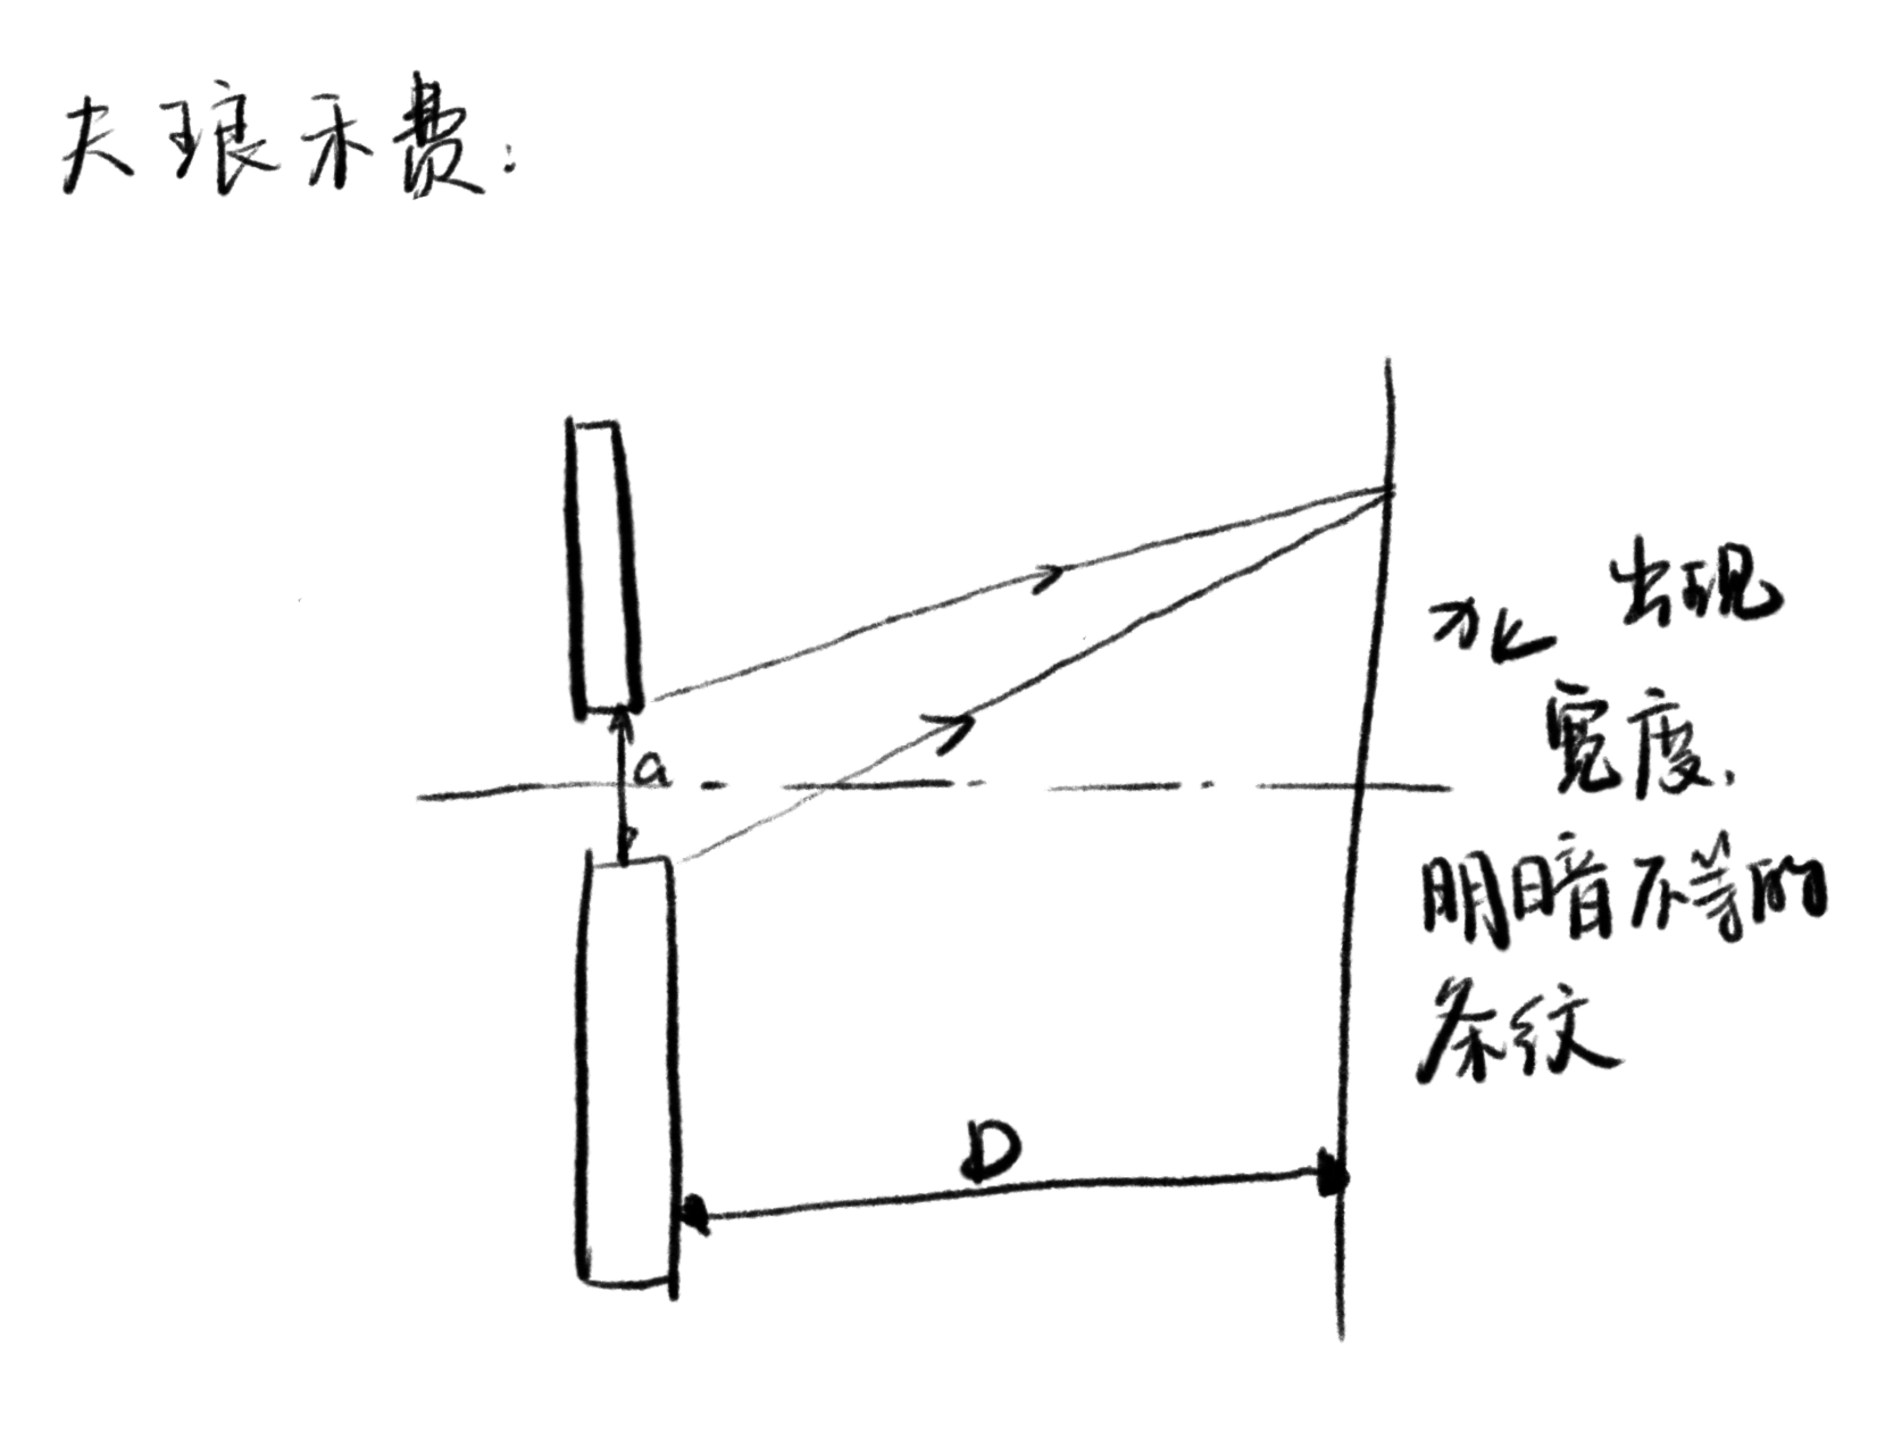
\includegraphics[width=.5\textwidth]{夫.pdf}
    \caption{夫琅禾费衍射}
\end{figure}

\paragraph{利用光栅衍射法测量激光波长}
光栅方程(主极大条件):
\[
d\sin \theta = \pm k\lambda(k = 0, \pm 1, \pm 2, \cdots)
\]
角度较小时,我们有$\sin\theta \approx \tan \theta \approx \frac{x}{D}$,即
\[
x_k = k\frac{D}{d}\lambda
\]
最后由公式\[\frac{x_1 - x_{-1}}{2} \approx \frac{D}{d}\lambda\]
可以求出激光波长
\begin{figure}[H]
    \centering
    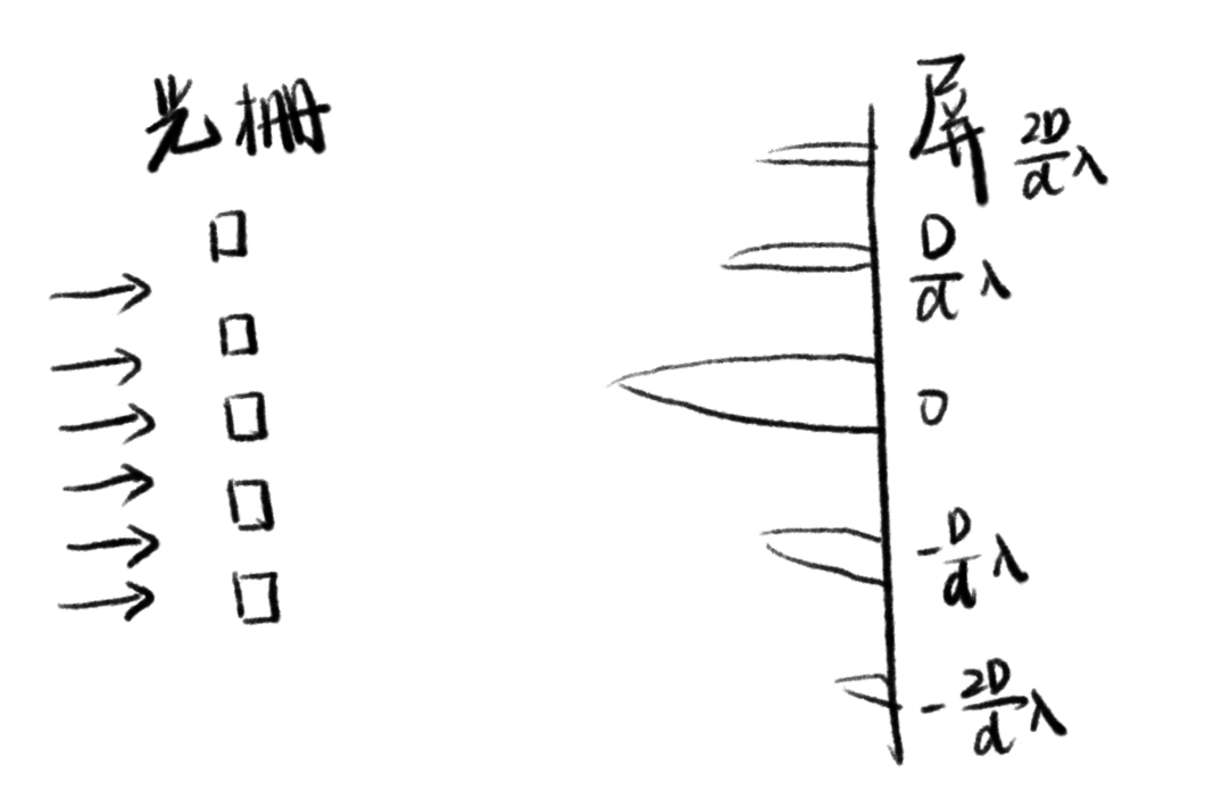
\includegraphics[width=.3\textwidth]{光栅.pdf}
    \caption{光栅衍射法测光的波长}
\end{figure}
\subsubsection{实验方法}
\begin{enumerate}
    \item \textbf{光路调节与校准:}
    调节光学导轨上的各个光学元件,确保它们的位置共轴且等高,以形成一条清晰、水平的实验光路。

    \item \textbf{观察不同孔隙的衍射图样:}
    将具有不同形状孔隙的衍射板置于光路中,定性观察并记录各自产生的夫琅禾费衍射图样的形状特征。

    \item \textbf{利用一维光栅测定激光波长:}
    使用一维光栅(已知参数为 50 条/\si{\mm})进行衍射实验。精确测量其衍射图样中正一级与负一级主极大亮纹之间的距离,然后依据光栅方程 $\frac{x_1 - x_{-1}}{2} \approx \frac{D}{d}\lambda$ 计算出所用激光的波长 $\lambda$。

    \item \textbf{研究单缝衍射的光强分布并测量缝宽:}
    观察由单缝产生的夫琅禾费衍射条纹。利用一维光强测量仪测出其光强分布。绘制出相对光强 $I/I_0$ 随位置坐标 $x$ 变化的函数图像,并根据衍射图样中暗纹的位置,计算出该单缝的精确宽度 $a$。

\end{enumerate}
\subsection{实验重点(3分)}
(简述本实验的学习重点,不超过100字。)
\begin{enumerate}
    \item \textbf{分析衍射图案:}首先要搞清楚,当光线通过不同形状的物体时,产生的衍射花样的明暗分布有什么不同和规律。
    \item \textbf{应用衍射原理进行测量:}要学会并熟练运用光的衍射,去测量一些微小量
    \item \textbf{了解更复杂的衍射:}最后,还需要了解当光通过二维光栅时,会产生怎样的衍射特征。
\end{enumerate}
\subsection{实验难点(2分)}
(简述本实验的实现难点,不超过100字。)
\begin{enumerate}
    \item 实验开始前需要调整光学导轨,确保各光学元件等高
    \item 读数需要小心,计算$D$的时候,接收屏位置$L_2$并非读数
    \item 转动轮毂时为了避免空程差,不能往回传,只能单向转动
    \item 测量的时候不能移动光学仪器的位置
\end{enumerate}
\begin{fullreportonly}
\section{原始数据(20分)}
(将有老师签名的“自备数据记录草稿纸”的扫描或手机拍摄图粘贴在下方,完整保留姓名,学号,教师签字和日期。)

\section{结果与分析(60分)}
\subsection{数据处理与结果(30分)}
(列出数据表格、选择适合的数据处理方法、写出测量或计算结果。)

\subsection{误差分析(20分)}
(运用测量误差、相对误差或不确定度等分析实验结果,写出完整的结果表达式,并分析误差原因。)

\subsection{实验探讨(10分)}
(对实验内容、现象和过程的小结,不超过100字。)

\section{思考题(10分)}
(解答教材或讲义或老师布置的思考题,请先写题干,再作答。)
\end{fullreportonly}
\insertnotes
\end{document}